%Authors guidlines: http://royalsocietypublishing.org/instructions-authors
% 2500 words max (includes the title page, abstract, references, acknowledgements and figure/table legends)
% current version is around 3700. I think a big cut down can be done on the references.
% We allow a maximum of 4 displays, only 2 of which can be figures.

\documentclass[12pt,letterpaper]{article}


%Packages
\usepackage{pdflscape}
\usepackage{fixltx2e}
\usepackage{textcomp}
\usepackage{fullpage}
\usepackage{float}
\usepackage{latexsym}
\usepackage{url}
\usepackage{epsfig}
\usepackage{graphicx}
\usepackage{amssymb}
\usepackage{amsmath}
\usepackage{bm}
\usepackage{array}
\usepackage[version=3]{mhchem}
\usepackage{ifthen}
\usepackage{caption}
\usepackage{hyperref}
\usepackage{amsthm}
\usepackage{amstext}
\usepackage{enumerate}
\usepackage[osf]{mathpazo}
\usepackage{dcolumn}
\usepackage{lineno}
\usepackage{longtable}
\pagenumbering{arabic}

\newcolumntype{L}[1]{>{\raggedright\let\newline\\\arraybackslash\hspace{0pt}}m{#1}}
\newcolumntype{C}[1]{>{\centering\let\newline\\\arraybackslash\hspace{0pt}}m{#1}}
\newcolumntype{R}[1]{>{\raggedleft\let\newline\\\arraybackslash\hspace{0pt}}m{#1}}

%Pagination style and stuff % NC: Note that these are all syst biol specific.
\linespread{2}
\raggedright
\setlength{\parindent}{0.5in}
\setcounter{secnumdepth}{0} 
\renewcommand{\section}[1]{%
\bigskip
\begin{center}
\begin{Large}
\normalfont\scshape #1
\medskip
\end{Large}
\end{center}}
\renewcommand{\subsection}[1]{%
\bigskip
\begin{center}
\begin{large}
\normalfont\itshape #1
\end{large}
\end{center}}
\renewcommand{\subsubsection}[1]{%
\vspace{2ex}
\noindent
\textit{#1.}---}
\renewcommand{\tableofcontents}{}
%\bibpunct{(}{)}{;}{a}{}{,}

%---------------------------------------------
%
%       START
%
%---------------------------------------------

\begin{document}


\newcommand{\beginsupplement}{%
    \setcounter{table}{0}
    \renewcommand{\thetable}{S\arabic{table}}%
    \setcounter{figure}{0}
    \renewcommand{\thefigure}{S\arabic{figure}}%
}

%Running head
\begin{flushright}
Version dated: \today
\end{flushright}

\bigskip
\medskip
\begin{center}

\noindent{\Large \bf Assessment of available anatomical characters for phylogenetic analysis among living mammals}

\bigskip
\noindent{\Large \bf Electronic Supplementary Material 2}

\bigskip
\noindent {\normalsize \sc Thomas Guillerme$^1$$^,$$^*$ and Natalie Cooper$^1$$^,$$^2$}\\
\noindent {\small \it 
$^1$School of Natural Sciences, Trinity College Dublin, Dublin 2, Ireland.\\
$^2$Department of Life Sciences, Natural History Museum, Cromwell Road, London, SW7 5BD, UK.}\\
\medskip
\noindent{*\bf Corresponding author.} \textit{t.guillerme@imperial.ac.uk}\\  
\vspace{1in}

\end{center}
%\modulolinenumbers[1]
%\linenumbers


\newpage


%TG: Maybe useless, I'll add that just in the thesis.
%\section{Graphical abstract}

%\begin{figure}[!htbp]
%\centering
%    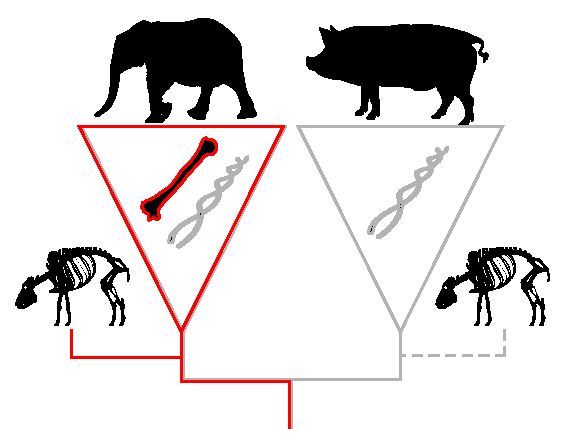
\includegraphics[width=1\textwidth]{MissingDataFigure.pdf}
%\caption{Example of topological errors due to missing morphological data in living taxa.
%The phylogeny contains two clades, Aves and Mammalia, with molecular data (grey) for both but only morphological data (red) for Aves.
%If a mammalian fossil species (with no molecular data) is added to the phylogeny, it will erroneously branch with the Aves instead of the Mammalia because no morphological data will overlap between the fossil mammals and the living ones.}
%\label{Figure_missing_data_problem}
%\end{figure}


\section{Supplementary results - 1}
The following section contains a supplementary analysis looking at the sampling effort for all the mammalian orders at the three different taxonomic levels (family, genus and species).
We calculated linear regressions %TG: does one calculate regressions? I would go for drawing regressions but that's not semantically correct...
between the logged number of sampled taxonomic levels per order against the logged total number of total taxonomic levels and fixed the intercept to 0.
This way we could calculate the slope of the regressions (\textit{b}) indicating the sampling effort (i.e. if the slope is 1, the sampling effort is maximum along each order for the taxonomic level, if 0 there is no significant sampling) and the fit of the regressions (\textit{R$^2$}).
The code for this analysis is available at this link \url{https://github.com/TGuillerme/Missing_living_mammals/blob/master/Analysis/Sampling_effort.R}.

\begin{figure}[!htbp]
\centering
    \includegraphics[width=1\textwidth]{Supp_figure_sampling_effort.pdf}
\caption{Sampling effort across all mammalian orders on the three different taxonomic levels. The \textit{R$^2$} and the slope (\textit{b}) are reported for each linear model.}
\label{Supp_Figure_sampling}
\end{figure}

This analysis shows suggests that the sampling effort reflects diversity for each taxonomic level (i.e. morphological characters were collected for each order according to it's size; Figure \ref{Supp_Figure_sampling}).
However, it is worth noting that this relation is stronger at higher taxonomic level (i.e. family, \textit{R$^2$}=0.99 \textit{b}=0.936) in comparison to the species level (\textit{R$^2$}=0.852 \textit{b}=0.711).
These results might be simply due to the increase of elements between each taxonomic levels (i.e. number of species $>$ genera $>$ families)
Nonetheless it is probable that mammalian morphological phylogeneticists did actually focused on resolving higher level relationships among mammalian orders (see Table 1 in the main text).

\newpage

\section{Supplementary results - 2}
The following section contains supplementary results to the main body: the phylogenetic representation of the data availability per order (excluding Primates and Carnivora, present in the main body).

\begin{figure}[!htbp]
\centering
    \includegraphics[width=1\textwidth]{Supp_figure_AFROSORICIDA.pdf}
\caption{Distribution of available morphological data across Afrosoricida. Edges are colored in grey when no morphological data is available or in blue when data is available.}
\label{Supp_Figure_Phylo-Afrosoricida}
\end{figure}

\begin{figure}[!htbp]
\centering
    \includegraphics[width=1\textwidth]{Supp_figure_CHIROPTERA.pdf}
\caption{Distribution of available morphological data across Chiroptera. Edges are colored in grey when no morphological data is available or in blue when data is available.}
\label{Supp_Figure_Phylo-Chiroptera}
\end{figure}

\begin{figure}[!htbp]
\centering
    \includegraphics[width=1\textwidth]{Supp_figure_CINGULATA.pdf}
\caption{Distribution of available morphological data across Cingulata. Edges are colored in grey when no morphological data is available or in blue when data is available.}
\label{Supp_Figure_Phylo-Cingulata}
\end{figure}

\begin{figure}[!htbp]
\centering
    \includegraphics[width=1\textwidth]{Supp_figure_DASYUROMORPHIA.pdf}
\caption{Distribution of available morphological data across Dasyuromorphia. Edges are colored in grey when no morphological data is available or in blue when data is available.}
\label{Supp_Figure_Phylo-Dasyuromorphia}
\end{figure}

\begin{figure}[!htbp]
\centering
    \includegraphics[width=1\textwidth]{Supp_figure_DIDELPHIMORPHIA.pdf}
\caption{Distribution of available morphological data across Didelphimorphia. Edges are colored in grey when no morphological data is available or in blue when data is available.}
\label{Supp_Figure_Phylo-Didelphimorphia}
\end{figure}

\begin{figure}[!htbp]
\centering
    \includegraphics[width=1\textwidth]{Supp_figure_DIPROTODONTIA.pdf}
\caption{Distribution of available morphological data across Diprotodontia. Edges are colored in grey when no morphological data is available or in blue when data is available.}
\label{Supp_Figure_Phylo-Diprotodontia}
\end{figure}

\begin{figure}[!htbp]
\centering
    \includegraphics[width=1\textwidth]{Supp_figure_ERINACEOMORPHA.pdf}
\caption{Distribution of available morphological data across Erinaceomorpha. Edges are colored in grey when no morphological data is available or in blue when data is available.}
\label{Supp_Figure_Phylo-Erinaceomorpha}
\end{figure}

\begin{figure}[!htbp]
\centering
    \includegraphics[width=1\textwidth]{Supp_figure_PILOSA.pdf}
\caption{Distribution of available morphological data across Pilosa. Edges are colored in grey when no morphological data is available or in blue when data is available.}
\label{Supp_Figure_Phylo-Pilosa}
\end{figure}

\begin{figure}[!htbp]
\centering
    \includegraphics[width=1\textwidth]{Supp_figure_CETARTIODACTYLA.pdf}
\caption{Distribution of available morphological data across Cetartiodactyla. Edges are colored in grey when no morphological data is available or in blue when data is available.}
\label{Supp_Figure_Phylo-Primates}
\end{figure}

\begin{figure}[!htbp]
\centering
    \includegraphics[width=1\textwidth]{Supp_figure_RODENTIA.pdf}
\caption{Distribution of available morphological data across Rodentia. Edges are colored in grey when no morphological data is available or in blue when data is available.}
\label{Supp_Figure_Phylo-Rodentia}
\end{figure}

\begin{figure}[!htbp]
\centering
    \includegraphics[width=1\textwidth]{Supp_figure_SCANDENTIA.pdf}
\caption{Distribution of available morphological data across Scandentia. Edges are colored in grey when no morphological data is available or in blue when data is available.}
\label{Supp_Figure_Phylo-Scandentia}
\end{figure}

\begin{figure}[!htbp]
\centering
    \includegraphics[width=1\textwidth]{Supp_figure_SORICOMORPHA.pdf}
\caption{Distribution of available morphological data across Soricomorpha. Edges are colored in grey when no morphological data is available or in blue when data is available.}
\label{Supp_Figure_Phylo-Soricomorpha}
\end{figure}


\end{document}